\documentclass{article}
\usepackage{amsmath,enumitem}
\usepackage{graphicx}
\usepackage{booktabs}
\usepackage{tabularx}
\usepackage[margin=1in]{geometry}
\usepackage{float}
\restylefloat{table}
\usepackage{placeins}
\usepackage[margin=1in]{geometry}


\begin{document}
	
	
\title{Econ 758 Assignment 1}
\author{Aaina Sharma and Randall Chicola}
\maketitle
\textbf{Empirical Application – Earned Income Tax Credit
} \\

\textbf{\underline{Question 1: Theoretical background and summary statistics}}

\begin{enumerate}
	
\item \textbf{Give a short description of the relevant aspects of the EITC expansion in 1993. (Hint: Have a look at Eissa and Hoynes, 2004.) Briefly discuss the theoretical predictions for the impact of the reform on the labor market participation of single women with children. You do not need to present a formal model!}\\

\textit{Answer: The EITC after its inception in 1975 as a payroll tax offset for low income families changed little until the TRA86 expansion in 1986, with continued expansion in 1990 OBRA90, and 1993 OBRA93.} \\

\textit{According to the Congressional Research Service's "The Earned Income Tax Credit (EITC): An Overview", the Clinton administration advocated the expansion to give incentive to "make work pay" for low income families with at least one full time working member making minimum wage.}\\

\textit{The were several material changes to the qualifying parameters of the EITC. Firstly, the maximum credits credit rates (maximum amount of qualified income for computing the credit) increased for a one child family from 23\% to 34\% in 1996. A family with two or more children saw a credit rate increase from 25\% to 40\%. Secondly, there was a lowering of the phase out range, 16.43\% to 15.98\% for one child families but the phaseout was increased from 17.86\% to 21.06\%.}\\

\textit{This would indicate that while the increase increases the slope for families of all size in the Phase-in region gives greater incentive to work, it appears divergent incentives may have been created for families with one child versus two or more children. Just as the steeper slope in the phase out region gives incentive to work, the shallower slope in the phase out region is to mitigate the negative substitution and income effects.} \\

\textit{While one child families were given incentive to work less as the amount of qualified income decreased in the phase out region which effectively increased there marginal tax rate when earning income beyond the phase-out threshold. Conversely, the increase in the rate applied to qualified income for families with two or more children provides less penalty for increasing income which would encourage labor force participation. } \\

\textit{Theoretical predictions of the re-form's impact on labor force participation of single women with children would be positive since a single taxpayer who still does not work as well those who prefer to work regardless have not changed their behavior. Those taxpayers on the the margin, may find the additional EITC income a sufficient inducement to enter the labor force.}


\item \textbf{Would you expect the number of children to influence the size of the effect? Why or why not? Explain.}

\textit{Answer: Since the number of eligible children is one of the parameters in  determining amount and eligibility of the EITC tax credit, more children resulting in a larger credit, it would not be surprising for the size of the effect to be influenced, which would allow for there to be identification between the groups of EITC participants. }

\item \textbf{Generate a table with descriptive statistics (Table 1, structured as in Table I in Eissa and Liebman, 1996), which contains the sample means of the variables nonwhite age ed work earn for two groups: single women with and without children. You do not need to display the standard deviations. Briefly discuss the differences.}

\textit{Answer: }
\begin{table}[htbp]\centering
	\def\sym#1{\ifmmode^{#1}\else\(^{#1}\)\fi}
	\caption{Summary Statistics}
	\begin{tabular}{l*{4}{c}}
		\hline\hline
		&\multicolumn{1}{c}{(1)}&\multicolumn{1}{c}{(2)}&\multicolumn{1}{c}{(3)}&\multicolumn{1}{c}{(4)}\\
		&\multicolumn{1}{c}{Without Children}&\multicolumn{1}{c}{With Children}&\multicolumn{1}{c}{With One Child}&\multicolumn{1}{c}{With Two or More Children}\\
		\hline
		age         &       38.50         &       32.72         &       33.76         &       32.05         \\
		&                     &                     &                     &                     \\
		[1em]
		ed          &       8.549         &       9.001         &       8.992         &       9.007         \\
		&                     &                     &                     &                     \\
		[1em]
		nonwhite    &       0.516         &       0.665         &       0.596         &       0.709         \\
		&                     &                     &                     &                     \\
		[1em]
		children    &           0         &       2.097         &           1         &       2.801         \\
		&                     &                     &                     &                     \\
		[1em]
		work        &       0.574         &       0.466         &       0.538         &       0.421         \\
		&                     &                     &                     &                     \\
		[1em]
		earn        &     13760.3         &      7909.9         &      9928.3         &      6613.5         \\
		&                     &                     &                     &                     \\
		\hline
		\(N\)       &        5927         &        7819         &        3058         &        4761         \\
		\hline\hline
		\multicolumn{5}{l}{\footnotesize mean coefficients; \textit{t} statistics in parentheses}\\
		\multicolumn{5}{l}{\footnotesize \sym{*} \(p<0.05\), \sym{**} \(p<0.01\), \sym{***} \(p<0.001\)}\\
	\end{tabular}
\end{table}





\item \textbf{Now calculate the sample means separately for single women with one child and women with two or more children (add the information to Table 1). How do they differ from each other?}

\textit{Answer: See above table }

\end{enumerate}


\textbf{\underline{Question 2: Difference-in-differences analysis}}\\

\bigskip
For the following analysis you need to generate two dummy variables to identify the treatment group (single women with children) [call it child] and the post-treatment period (1994-1996) [call it post1993].


\begin{enumerate}
	
	\item \textbf{Create a figure (Figure 1) that illustrates the annual mean labor market participation rates by year (1991-1996) for single women with children (treatment group) and single women without children (control group). Label the axes and include a title and a legend into the graph.}

\textit{Answer: }

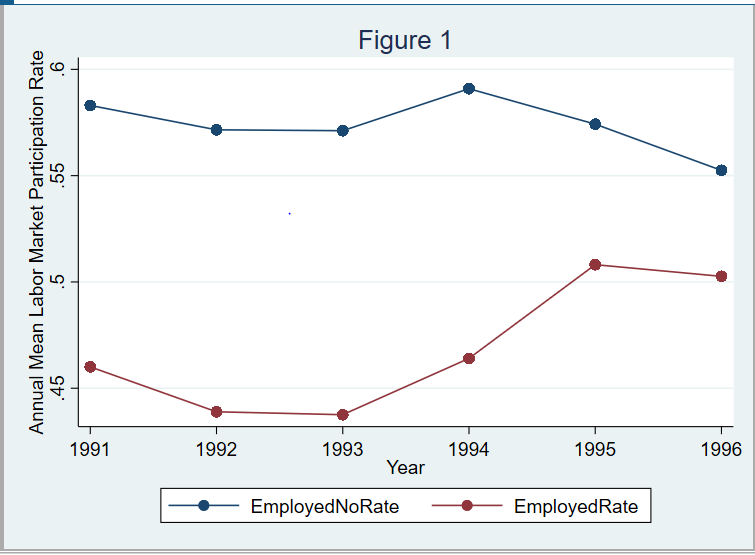
\includegraphics[width = \textwidth]{Figure 1.png}



\item \textbf{Now normalize the value of the labor force participation rate for each of the two groups to group-specific 1991 values. That is, the mean of the labor market participation rates in 1991 become equal to 1. Plot a graph (as the one before, including labeling, title, and legend) in Figure 2.}

\textit{Answer: }

\item \textbf{Based on Figures 1 and 2, discuss the validity of using single women without children as control group.   }


\textit{Answer: }



\item \textbf{ Calculate the sample means of labor force participation rates (work) of women with and without children for the pre- (average over 1991-1993) and post-reform (average over 1994-1996) period. Organize your table (Table 2) as in Table II in Eissa and Liebman (1996).  }


\textit{Answer: }

\item \textbf{  Calculate the within- and between-group differences as well as the unconditional difference-in-differences estimate and add them to Table 2. Briefly comment on your results. }


\textit{Answer: }

\item \textbf{ Repeat the comparison separately for women with one child and for women with at least two children for the years before and after the EITC expansion. Again compute the within- and between-group differences and the difference-in-differences estimates. Compare each of the two groups separately to single women without children (the control group). Display the results in Table 3 and discuss your findings. For which of the two groups do you find larger treatment effects? Is this consistent with the theoretical predictions?  }


\textit{Answer: }

\item \textbf{ Return to the comparison of women with and without children. Estimate the difference-in-differences effect from the EITC expansion by running OLS regressions. As dependent variable, use the dummy indicating labor market participation (work). First run a regression without controls (“unconditional diff-in-diff estimate”). Then add control variables (urate nonwhite age ed) to obtain the “conditional diff-in-diff estimate”. Present your results (including standard errors) in Table 4 and interpret them. Compare the estimates and their statistical significance for the conditional and unconditional difference-in-differences estimates. Also comment on the estimated coefficients of child and post1993.  }


\textit{Answer: }

\item \textbf{  Estimate a conditional (i.e., including urate nonwhite age ed), “placebo” treatment model on the pre-treatment period. For this purpose, take data from the years 1991-1993 only and leave the treatment and control groups unchanged. Assume for the analysis that the placebo reform would have taken place on January 1st, 1992 (generate a dummy variable postplacebo that is one for year 1992 and after and an interaction with child) and present your results (including standard errors) in Table 5. What do you find, and how do you interpret this? }



\end{enumerate}



\end{document}
